\documentclass[11pt]{article}
\usepackage[a4paper,margin=1in]{geometry}
\usepackage{amsmath,amssymb,amsthm,mathtools}
\usepackage{booktabs}
\usepackage{array}
\usepackage{enumitem}
\usepackage{float}
\usepackage{graphicx}
\usepackage{hyperref}
\usepackage[nameinlink,capitalise]{cleveref}
\usepackage[numbers,sort&compress]{natbib}

\newtheorem{theorem}{Theorem}[section]
\newtheorem{proposition}[theorem]{Proposition}
\newtheorem{corollary}[theorem]{Corollary}
\newtheorem{remark}[theorem]{Remark}
\theoremstyle{definition}
\newtheorem{definition}[theorem]{Definition}
\newcommand{\norm}[1]{\left\lVert#1\right\rVert}
\newcommand{\F}{\mathrm F}
\newcolumntype{L}[1]{>{\raggedright\arraybackslash}p{#1}}

\title{Validated Upstream-to-Frozen Hardy Bridges for the Folded-Gaussian Production Chain\\
\large Analytic Factor Transport, Normalized Couplings, and a Robust Four-Block Difference Tail}
\author{Liang Wang}
\date{July 2026}

\begin{document}
\maketitle

\begin{abstract}
RH-70 certified terminal Hardy bounds for exact-dyadic frozen production
arrays, but folded-Gaussian assembly, spectral deflation, and normalized
source/observation construction remained upstream of that certificate.  RH-72
and RH-73 supplied the missing matrix and peripheral-factor balls.  This paper
composes those balls through the production formulas and closes the complete
finite-scale upstream-to-frozen bridge.

First, a norm-bounded perturbation of the repaired matrix is propagated through
the stationary Neumann system, the bordered right-eigenpair Newton map, and the
bordered left solve.  This validates Perron/parity projectors and deflated bulk
operators for the analytic folded-Gaussian midpoint matrices themselves.  For
nonzero coupling blocks $B,B_0$, we use
\[
 \norm{B/\norm B_{\F}-B_0/\norm{B_0}_{\F}}_{\F}
 \le \frac{2\varepsilon}{\norm{B_0}_{\F}-\varepsilon},
 \qquad \norm{B-B_0}_{\F}\le\varepsilon<\norm{B_0}_{\F},
\]
and product perturbation bounds to enclose every operator, source, and
observation against its RH-70 frozen counterpart.

Second, let $A=A_0+E$, $\norm E\le\varepsilon_A$, and
$C_k\ge\norm{A_0^k}$.  The discrete Volterra identity gives the rigorous
recursion
\[
 D_k=\varepsilon_A\sum_{j=0}^{k-1}C_{k-1-j}(C_j+D_j)
 \ge\norm{A^k-A_0^k}.
\]
This bounds every finite transfer-coefficient difference.  A common block
horizon certifies both $A^M$ and $A_0^M$ contractive; four block lengths then
leave a geometric true/reference tail.  The result is a robust realization of
the augmented Hardy difference bridge.

A 160-bit Arb audit covers both left and right channels at
$\sigma=0.16,0.08,0.04,0.02,0.01$.  The largest certified operator, source,
and observation errors are $2.64\times10^{-11}$,
$2.63\times10^{-11}$, and $1.74\times10^{-11}$.  The largest full Hardy
bridge is $2.03\times10^{-6}$.  Every bridge lies below its inherited RH-71
one-percent headroom; the worst consumes only $0.217\%$ of that slack.

Thus the five archived scales are now green from analytic folded-Gaussian
assembly through rank-two deflation and terminal Hardy completion.  This is a
finite-scale closure, not a uniform small-noise theorem: Stage A1 and
unconditional Stage A4 remain open, as do all later Hilbert--Polya and
Riemann-Hypothesis objectives.
\end{abstract}

\noindent\textbf{Keywords:} Hardy norm; interval arithmetic; spectral
projector; normalized coupling; Volterra identity; robust systems.

\medskip
\noindent\textbf{MSC 2020:} 47A10; 47A55; 47B35; 65G20; 93B28.

\section{Introduction}

The production chain used in the recent RH layers has four stages:
\begin{equation}
 \text{folded kernel}
 \longrightarrow \text{Perron/parity deflation}
 \longrightarrow \text{normalized transfer blocks}
 \longrightarrow \text{Hardy completion}.
 \label{eq:chain}
\end{equation}
RH-70 proved the last arrow rigorous after the generated binary64 arrays were
embedded as exact dyadic Arb inputs \citep{WangFrozen2026}.  Its result was
therefore ``frozen green'' but ``end-to-end amber.''  RH-71 quantified the
remaining upstream bridge budget: all ten channels retain positive headroom
inside a one-percent finite-scale target \citep{WangReview2026}.

RH-72 certified the analytic folded-Gaussian midpoint matrices against exact
stochastic dyadic repairs, including Haar coarse and cross blocks
\citep{WangAssembly2026}.  RH-73 then validated the stationary and negative
parity factors of those repaired matrices \citep{WangPeripheral2026}.  Two
tasks remain before these results can be inserted into RH-70:

\begin{enumerate}[leftmargin=2.2em]
 \item transfer the repaired spectral factors across the RH-72 analytic
       matrix ball and through all source/observation normalizations;
 \item certify the Hardy norm of the difference between every resulting
       analytic transfer sequence and the frozen sequence.
\end{enumerate}

The first task is delicate because projectors and normalized couplings are
nonlinear.  The second cannot use a one-step geometric estimate: the scaled
bulk matrices are stable but nonnormal, and their one-step Euclidean norms
need not be below one.  The correct object is the already certified block
contraction.

This paper supplies both pieces.  All binary64 arrays serve only as exact
dyadic centers.  Scalar decisions and matrix products used by the certificate
are recomputed at 160-bit Arb precision \citep{Johansson2017,Higham2002}.

\section{The analytic and frozen triples}
\label{sec:triples}

Let $P_f$ be the analytic fine folded-Gaussian midpoint matrix and let $U,W$
be the exact Haar coarse and detail embeddings.  Define
\[
 P_c=U^TP_fU,qquad B=U^TP_fW,qquad C=W^TP_fU.
\]
For either fine or coarse matrix, let $\Pi_+$ and $\Pi_-$ denote its Perron and
negative parity Riesz projectors, let $\lambda_-$ be the parity eigenvalue, and
put
\[
 Q=I-\Pi_+-\Pi_-,qquad
 K=P-\Pi_+-\lambda_-\Pi_-.
\]

At the fixed Hardy radius $R_H=0.85$, the true left and right production
triples are
\begin{align}
 A_L&=K_f/R_H,&
 X_L&=Q_fU\frac{B}{\norm B_{\F}},&
 Y_L&=U^T,\label{eq:left}\\
 A_R&=K_c^T/R_H,&
 X_R&=\frac{C^T}{\norm C_{\F}},&
 Y_R&=Q_c^T.\label{eq:right}
\end{align}
The frozen triples $(A_{0,s},X_{0,s},Y_{0,s})$ use the RH-70 binary64 matrix,
Haar constant, eigendecomposition, and normalizations, interpreted as exact
dyadic arrays.

Our goal is to certify
\[
 \norm{A_s-A_{0,s}}_2\le\varepsilon_{A,s},
 \quad
 \norm{X_s-X_{0,s}}_{\F}\le\varepsilon_{X,s},
 \quad
 \norm{Y_s-Y_{0,s}}_{\F}\le\varepsilon_{Y,s},
 \label{eq:triple-errors}
\]
and then bound the full transfer difference
\begin{equation}
 \Delta_s^2
 =\sum_{k\ge0}
 \norm{Y_sA_s^kX_s-Y_{0,s}A_{0,s}^kX_{0,s}}_{\F}^2.
 \label{eq:bridge}
\end{equation}

\section{Transporting repaired factors to the analytic matrix}
\label{sec:factors}

Let $A_r$ be an exact repaired stochastic matrix and let
$A=A_r+E$, $\norm E_2\le\delta$, be the corresponding analytic matrix.
RH-73 provides stationary and parity centers together with inverse,
residual, and contraction bounds for $A_r$.

\subsection{Stationary factor}

Let
\[
 L_r=I-A_r^T+\frac1n\mathbf1\mathbf1^T,
 \qquad L=L_r-E^T.
\]
If $M_r\ge\norm{L_r^{-1}}$ and $M_r\delta<1$, then
\begin{equation}
 \norm{L^{-1}}
 \le\frac{M_r}{1-M_r\delta}.
 \label{eq:stationary-transfer}
\end{equation}
If the repaired stationary vector obeys
$\norm{\pi_r-\pi_0}\le e_r$, subtraction of $L\pi=L_r\pi_r=n^{-1}\mathbf1$
gives
\begin{equation}
 \norm{\pi-\pi_0}
 \le e_r+
 \frac{M_r\delta(\norm{\pi_0}+e_r)}{1-M_r\delta}.
 \label{eq:stationary-ball}
\end{equation}
Since the analytic matrix is exactly stochastic, its Perron right vector is
again $\mathbf1$ and the projector error is $\sqrt n$ times
\eqref{eq:stationary-ball}.

\subsection{Bordered parity factors}

For the RH-73 right Newton system, let $\beta,\gamma,M$ be the repaired
preconditioned residual, Jacobian defect, and inverse norm.  The matrix ball
augments them to
\begin{equation}
 \widehat\beta=\beta+M\delta\norm{r_0},qquad
 \widehat\gamma=\gamma+M\delta.
 \label{eq:augmented-newton}
\end{equation}

\begin{proposition}[Analytic bordered eigenpair ball]
\label{prop:right}
If
\[
 \widehat\beta+\widehat\gamma\rho+M\rho^2\le\rho,
 \qquad \widehat\gamma+M\rho<1,
\]
then every matrix in the norm ball, in particular $A$, has a unique normalized
right parity eigenpair in the joint radius-$\rho$ ball around the archived
center.
\end{proposition}

\begin{proof}
The perturbation contributes $Er_0$ to the center residual and $E$ to the
right-vector block of the Jacobian.  Their preconditioned norms are bounded by
the two added terms in \eqref{eq:augmented-newton}.  The bilinear remainder is
unchanged, so the RH-73 contraction proof applies uniformly over the matrix
ball.
\end{proof}

For the bordered left system, matrix and eigenvalue perturbations contribute
at most $M_\ell(\delta+\rho)$.  Thus, with repaired defect $\gamma_\ell$,
inverse norm $M_\ell$, center residual correction $\beta_{\ell,0}$, and left
center norm $L_0$, we use
\begin{align}
 \Gamma_\ell&=\gamma_\ell+M_\ell(\delta+\rho),\label{eq:left-defect}\\
 e_\ell&=
 \frac{\beta_{\ell,0}+M_\ell(\delta+\rho)L_0}{1-\Gamma_\ell}.
 \label{eq:left-ball}
\end{align}
Every archived channel has $\Gamma_\ell<1$.  RH-73's normalized projector
formula then gives analytic $\Pi_-$, rank-two, complement, and bulk balls.  The
bulk bound additionally contains the base matrix error $\delta$.

\section{Normalized source/observation transfer}
\label{sec:normalization}

\begin{proposition}[Normalized coupling perturbation]
\label{prop:normalization}
Let $B_0\ne0$ and suppose
$\norm{B-B_0}_{\F}\le\varepsilon<\norm{B_0}_{\F}$.  Then
\begin{equation}
 \norm{B/\norm B_{\F}-B_0/\norm{B_0}_{\F}}_{\F}
 \le\frac{2\varepsilon}{\norm{B_0}_{\F}-\varepsilon}.
 \label{eq:normalized}
\end{equation}
\end{proposition}

\begin{proof}
Insert $B_0/\norm B_{\F}$ and use
$|\norm B_{\F}-\norm{B_0}_{\F}|\le\varepsilon$ and
$\norm B_{\F}\ge\norm{B_0}_{\F}-\varepsilon$.
\end{proof}

RH-72 gives a common two-norm error $e_H$ for exact analytic coarse and cross
blocks against the frozen pipeline.  For an $m\times m$ block,
\begin{equation}
 \norm{B-B_0}_{\F},\ \norm{C-C_0}_{\F}le\sqrt m\,e_H.
 \label{eq:cross-frob}
\end{equation}
It also gives $\norm{U-U_0}_2\le e_U$ and hence
$\norm{U-U_0}_{\F}\le\sqrt m,e_U$.

For example, if $e_Q\ge\norm{Q_f-Q_{f,0}}_2$ and
$N_{Q,0}\ge\norm{Q_{f,0}}_2$, the left source obeys
\begin{equation}
 \norm{X_L-X_{L,0}}_{\F}
 \le e_Q+N_{Q,0}e_U
 +N_{Q,0}\norm{U_0}_2 e_{\widehat B},
 \label{eq:left-source}
\end{equation}
where $e_{\widehat B}$ is the right side of \eqref{eq:normalized}.  The right
source error is $e_{\widehat C}$, the left observation error is
$\sqrt m,e_U$, and the right observation error is the Frobenius complement
ball.  Together with the bulk bounds, these are exactly the triple errors in
\eqref{eq:triple-errors}.

\section{A robust augmented Hardy difference bridge}
\label{sec:hardy}

Fix one channel and suppress its subscript.  Write $A=A_0+E$ and let
$\norm E_2\le\varepsilon_A$.  Suppose $C_k\ge\norm{A_0^k}_2$.

\begin{theorem}[Volterra power perturbation]
\label{thm:volterra}
Define $D_0=0$ and
\begin{equation}
 D_k=\varepsilon_A
 \sum_{j=0}^{k-1}C_{k-1-j}(C_j+D_j).
 \label{eq:volterra}
\end{equation}
Then $\norm{A^k-A_0^k}_2\le D_k$ and
$\norm{A^k}_2\le C_k+D_k$ for every $k$.
\end{theorem}

\begin{proof}
The discrete Volterra identity is
\[
 A^k-A_0^k
 =\sum_{j=0}^{k-1}A_0^{k-1-j}EA^j.
\]
Induction and submultiplicativity give \eqref{eq:volterra}.
\end{proof}

Let $x_0=\norm{X_0}_{\F}$, $y_0=\norm{Y_0}_{\F}$, and let
$\varepsilon_X,\varepsilon_Y$ be the source and observation errors.  Put
$x=x_0+\varepsilon_X$.  From a three-term expansion of the transfer
coefficient,
\begin{equation}
 \begin{split}
 d_k:={}&\varepsilon_Y(C_k+D_k)x\\
 &+y_0\{D_kx+C_k\varepsilon_X\}
 \end{split}
 \label{eq:coefficient}
\end{equation}
bounds
$\norm{YA^kX-Y_0A_0^kX_0}_{\F}$.

The reference block horizon $M$ is inherited from RH-70.  Arb computes exact
dyadic prefix power bounds $C_r$ for $0\le r\le M$ and
$q_0=C_M<1$.  For $k=bM+r$, we use
\begin{equation}
 C_k=q_0^bC_r.
 \label{eq:block-powers}
\end{equation}
Let $q=C_M+D_M<1$, and let $S,S_0$ bound the true and reference source-state
energies over one block.

\begin{theorem}[Robust four-block Hardy bridge]
\label{thm:bridge}
For any integer $b\ge1$,
\begin{equation}
 \begin{split}
 \Delta^2\le{}&\sum_{k=0}^{bM-1}d_k^2\\
 &+2(y_0+\varepsilon_Y)^2
   \frac{q^{2b}}{1-q^2}S
 +2y_0^2\frac{q_0^{2b}}{1-q_0^2}S_0.
 \end{split}
 \label{eq:bridge-upper}
\end{equation}
\end{theorem}

\begin{proof}
The finite prefix follows from \eqref{eq:coefficient}.  After $b$ blocks, the
true and reference state blocks contract geometrically by $q$ and $q_0$.
The squared norm of their transfer difference is at most twice the sum of the
two squared norms.  Summing both geometric tails proves
\eqref{eq:bridge-upper}.
\end{proof}

This theorem is the uncertainty-robust form of RH-70's augmented difference
bridge.  The exact block-diagonal realization identifies the transfer
difference; \cref{thm:volterra,thm:bridge} enclose every realization allowed by
the upstream triple balls without replacing those balls by independent
entrywise intervals.

\section{Five-scale interval audit}
\label{sec:audit}

The implementation uses $b=4$ and 160-bit Arb arithmetic.  All repaired and
frozen entries are exact rationals; all center differences, row/column sums,
Frobenius norms, factor-transfer denominators, normalized-coupling
denominators, Volterra recursions, finite energies, and tails are outward
rounded.

\begin{table}[H]
\centering
\small
\caption{Certified upstream triple errors.  Each row reports the larger of
the left and right channel values.}
\label{tab:triple}
\begin{tabular}{@{}rrrrr@{}}
\toprule
$\sigma$ & $n$ & $\varepsilon_A$ & $\varepsilon_X$ & $\varepsilon_Y$\\
\midrule
0.16 & 32  & $1.44\,10^{-13}$ & $2.86\,10^{-13}$ & $9.62\,10^{-14}$\\
0.08 & 64  & $4.22\,10^{-13}$ & $6.70\,10^{-13}$ & $2.89\,10^{-13}$\\
0.04 & 128 & $1.28\,10^{-12}$ & $1.70\,10^{-12}$ & $8.14\,10^{-13}$\\
0.02 & 256 & $5.68\,10^{-12}$ & $6.34\,10^{-12}$ & $3.70\,10^{-12}$\\
0.01 & 512 & $2.64\,10^{-11}$ & $2.63\,10^{-11}$ & $1.74\,10^{-11}$\\
\bottomrule
\end{tabular}
\end{table}

The growth is visible but remains tiny relative to every normalization and
block-contraction margin.  In particular, the largest true block-power upper
is $0.021022$.

\begin{table}[H]
\centering
\small
\caption{Full Hardy bridge upper, inherited one-percent slack, and percentage
of slack consumed.}
\label{tab:bridge}
\begin{tabular}{@{}rrrrrrr@{}}
\toprule
&\multicolumn{3}{c}{left}&\multicolumn{3}{c}{right}\\
\cmidrule(lr){2-4}\cmidrule(l){5-7}
$\sigma$ & bridge & slack & use & bridge & slack & use\\
\midrule
0.16 & $1.42\,10^{-6}$ & $5.82\,10^{-3}$ & $0.0245\%$ & $1.26\,10^{-6}$ & $6.81\,10^{-3}$ & $0.0185\%$\\
0.08 & $8.13\,10^{-7}$ & $6.98\,10^{-3}$ & $0.0117\%$ & $5.85\,10^{-7}$ & $8.73\,10^{-3}$ & $0.00670\%$\\
0.04 & $1.83\,10^{-6}$ & $8.42\,10^{-4}$ & $0.217\%$ & $2.03\,10^{-6}$ & $1.32\,10^{-3}$ & $0.155\%$\\
0.02 & $6.64\,10^{-7}$ & $1.08\,10^{-3}$ & $0.0617\%$ & $5.65\,10^{-7}$ & $3.60\,10^{-3}$ & $0.0158\%$\\
0.01 & $3.12\,10^{-7}$ & $2.11\,10^{-3}$ & $0.0149\%$ & $2.55\,10^{-7}$ & $3.63\,10^{-3}$ & $0.00704\%$\\
\bottomrule
\end{tabular}
\end{table}

Every channel therefore satisfies the RH-71 composition criterion
\[
 \Delta_s\le(1.01)F_s-U_s,
\]
where $F_s$ is the certified frozen finite-prefix lower and $U_s$ the frozen
full upper.  Combining the triangle inequality with RH-70 proves an
end-to-end one-percent finite-scale Hardy upper for the analytic production
triple.

\begin{figure}[H]
\centering
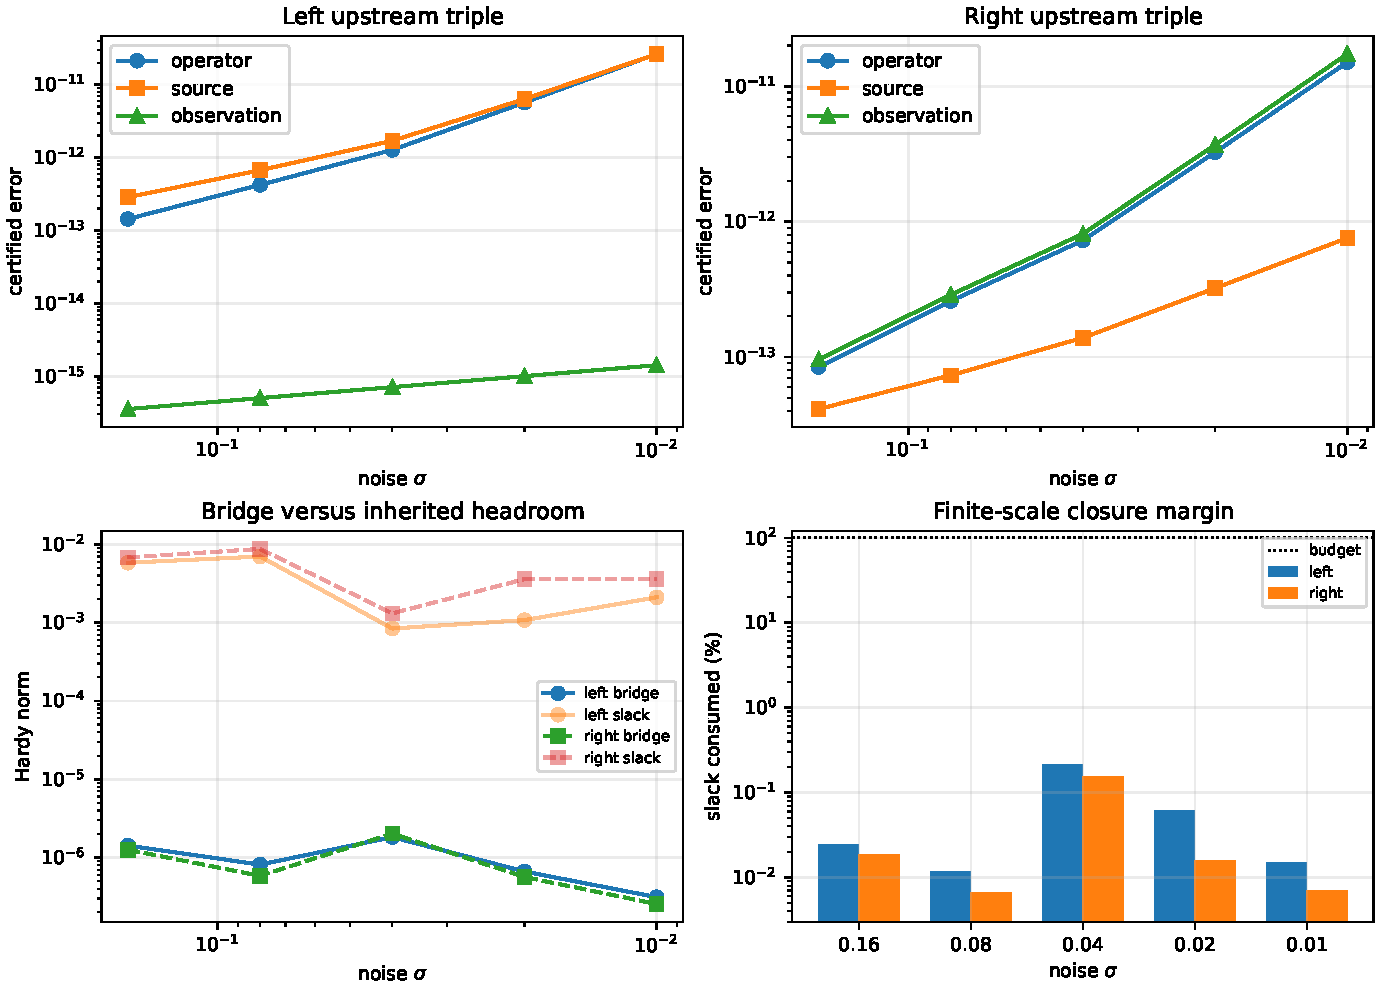
\includegraphics[width=0.98\textwidth]{figures/validated_upstream_hardy_bridge.pdf}
\caption{Certified triple errors, full upstream bridges versus inherited
headroom, and the fraction of slack consumed.}
\label{fig:audit}
\end{figure}

\section{Route consequence and claim boundary}
\label{sec:boundary}

The finite-scale chain \eqref{eq:chain} is now closed at all five archived
scales.  The result includes:

\begin{enumerate}[leftmargin=2.2em]
 \item analytic folded-Gaussian and Haar assembly;
 \item analytic Perron/parity factor transfer and rank-two deflation;
 \item normalized source/observation transfer;
 \item a robust augmented Hardy difference bridge;
 \item composition with the frozen terminal Hardy certificate.
\end{enumerate}

This changes the route map.  ``Upstream interval inclusion'' is no longer an
open finite-scale gate.  Full Stage A1 still requires a uniform theorem for
the small-noise/dyadic family: the archived dimensions, horizons, factor
condition numbers, and triple errors must be replaced by analytic functions
of $\sigma$ and the dyadic level.  The next papers should therefore study
uniform horizon, phase, and effective-rank scaling.

The present finite list does not close Stage A1, unconditional Stage A4, or a
renormalized determinant limit.  It constructs no self-adjoint
Hilbert--Polya operator, proves no $T\log T$ counting law or prime-power trace
formula, identifies no zeta zeros, and does not prove the Riemann Hypothesis.

\section{Conclusion}

The earlier amber status came from a genuine certificate boundary, not from a
large numerical discrepancy.  Once the RH-72 and RH-73 balls are propagated
through the exact production formulas, the complete upstream mismatch is only
of order $10^{-6}$ in Hardy norm and consumes at most $0.217\%$ of the
available bridge slack.  The finite-scale production chain is therefore
rigorous end to end.

The surviving wall is asymptotic.  RH-75 should begin replacing the five
observed block horizons by a uniform small-noise horizon law, while preserving
the blockwise mechanism that made the present closure possible.

\bibliographystyle{plainnat}
\bibliography{references}

\end{document}
